% !TeX spellcheck = en_US
\documentclass{article}
\usepackage{graphicx}
\usepackage{fancybox}
\usepackage{tikz}
\usepackage{algorithm}
\usepackage{amsmath}
\usepackage{algorithmicx}
\usepackage{algpseudocode}
\usepackage{graphicx}
\usepackage{hyperref}
\usepackage{enumitem}
\usepackage{fancybox}
\usepackage{tikz}
\usepackage{caption}

\captionsetup{labelfont={color=black,bf}}


\makeatletter
\def\BState{\State\hskip-\ALG@thistlm}
\makeatother

\algdef{SE}[DOWHILE]{Do}{doWhile}{\algorithmicdo}[1]{\algorithmicwhile\ #1}%

\title{Homework 05: Sorting (Part 2)}
\date{\today}
\author{Roberto Corti}

\begin{document}
	\maketitle
	
	\section*{Exercise 1}
	\textbf{Generalize the SELECT algorithm to deal also with repeated values and prove that it still belongs to $O(n)$.}
	
	\section*{Exercise 2}
	\textbf{Download the latest version of the code from}
	\begin{center}
		\url{https://github.com/albertocasagrande/AD_sorting}
	\end{center}
	\textbf{and} 
	\begin{itemize}
		\item \textbf{Implement the SELECT algorithm of Ex. 1.}
		\item \textbf{Implement a variant of the QUICK SORT algorithm using above mentioned SELECT to identify the best pivot for partitioning.}
		\item \textbf{Draw a curve to represent the relation between the input size and the execution-time of the two variants of QUICK SORT (i.e, those of Ex. 2 and Ex. 1 31/3/2020) and discuss about their complexities.}
	\end{itemize}

	\noindent The new version of SELECT that deals with repeated values described in the previous section is implemented inside the file \texttt{select.c} and \texttt{quick\_sort.c} for the tri-partition implementation.\\
	Once applied this algorithm, I implemented a variant of QUICK SORT using the SELECT method in order to choose the best pivot:
	
		\begin{algorithm}
		\texttt{Quick-Sort Select(A, left, right):} \label{ex2}
		\begin{algorithmic}
			\While {$\mathtt{left \space \leq \space right}$}
			\State \texttt{pivot} $\gets$ \texttt{select\_pivot(A, left, right)}
			\State \texttt{Quick-Sort  Select(A, left, k.first)}
			\State \texttt{left} $\gets$ \texttt{k.second+1}
			\EndWhile
			
		\end{algorithmic}
	\end{algorithm}

	\newpage
	
	\noindent The results, compared with the classic version of QUICK SORT, are represented in the following plot.
	
	\begin{figure}[h]
		\centering
		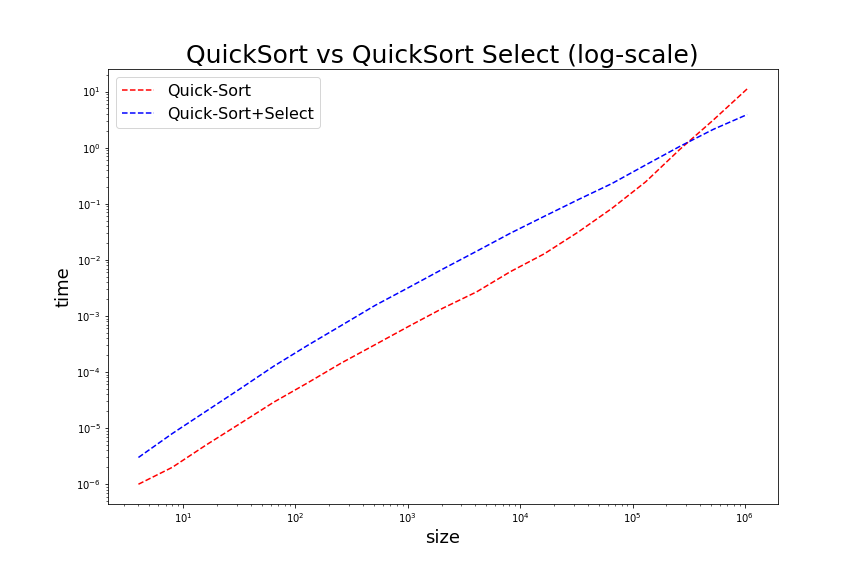
\includegraphics[width=.8\textwidth]{../plot/quicksort.png}  
		\caption{Benchmark of the \texttt{quick\_sort} method compared to its version when the \texttt{select} algorithm is involved in the selection of the pivot.}
		\label{plot}
	\end{figure}
	
	\noindent As it can be observed, the classic QUICK SORT has better performances on small list sizes. However, for big arrays the cost of partitioning becomes relevant and in those cases QUICK-SORT SELECT results to be more efficient.
	
	
	\section*{Exercise 3}
	\textbf{(Ex. 9.3-1 in [1]) In the algorithm SELECT, the input elements are divided into chunks of 5. Will the algorithm work in linear time if they are divided into chunks of 7? What about chunks of 3?} \\
	
	\noindent In the case of having divided into chunks of 7, as we did at lesson, we can get a lower bound on the number of elements that are greater than the median-of-median (say $\hat{m}$), that is 
	$$
	4 \bigg(\bigg\lceil \frac{1}{2} \Big\lceil \frac{n}{7} \Big\rceil \bigg\rceil
	- 2 \bigg) \ge \frac{2n}{7} - 8.
	$$
	Then, the upper bound for the number of elements smaller or equal to $\hat{m}$ is 
	$$
	n-\Big(\frac{2n}{7} - 8\Big) = \frac{5n}{7} +8,
	$$
	and this leads to the following recurrence:
	$$
	T_S(n)=T_S(\lceil n/7 \rceil) + T_S(5n/7 + 8) + \Theta(n).
	$$
	Selecting $cn$ and $c'n$ as representatives of $O(n)$ and $\Theta(n)$ and assuming that $T_S(m) \leq cm$ $\forall m < n$ 
	\begin{align}
	\nonumber
	T(n) & \le c\lceil n/7 \rceil + c(5n/7 + 8) + c'n \\
	\nonumber
	& \le cn/7 + c + 5cn/7 + 8c + c'n \\
	\nonumber
	& = 6cn/7 + 9c + c'n \\
	\nonumber
	& = cn + (-cn/7 + 9c + c'n). 
	\end{align}
	which is at most $cn$ if $ (-cn/7 + 9c + c'n) \le 0 $. This is equivalent to $ c \ge \frac{7c'n}{n - 63}$ and picking $n\geq 126$ and $c\geq 14c'$, we get $T_S(n) \leq cn$ and $T_S(n) \in O(n)$.
	\\
	
	If we divide in groups of 3, the number of elements that are greater than the median-of-medians $\hat{m}$ is:
	
	$$
	2 \bigg(\bigg\lceil \frac{1}{2} \Big\lceil \frac{n}{3} \Big\rceil \bigg\rceil
	- 2 \bigg) \ge \frac{n}{3} - 4,
	$$
	so the upper bound for the number of elements smaller or equal to $\hat{m}$ is 
	$$
	n-\Big(\frac{n}{3} - 4\Big) = \frac{2n}{3} +4.
	$$
	The recurrence is thus 
	$$
	T(n) = T(\lceil n/3 \rceil) + T(2n/3 + 4) + \Theta(n).
	$$
	We guess that $T(n)>cn$ and bounding the non-recursive term with $c'n$:
	\begin{align}
	\nonumber
	T(n) & > c\lceil n/3 \rceil + c(2n/3 + 2) + an \\
	\nonumber
	& > cn/3 + c + 2cn/3 + 2c + an \\
	\nonumber
	& = cn + 3c + an \\
	\nonumber
	& > cn ,
	\end{align}
	which holds for any $c>0$.
	\newpage
	\section*{Exercise 4}
	\textbf{(Ex. 9.3-5 in [1]) Suppose that you have a “black-box” worst-case linear-time subroutine to get the position in A of the value that would be in position $n/2$ if A was sorted. Give a simple, linear-time algorithm that
	solves the selection problem for an arbitrary position i.}\\

	\noindent Let $A$ be the array and denote by $i$ the arbitrary position. The black-box subroutine if applied to $A$ returns the $n/2$ element. If $i=n/2$ the problem is solved. Otherwise, we can partition $A$ into $A_1$, $A_2$ those elements are respectively lower and greater than $A[n/2]$. If $i<n/2$, we will call recursively the algorithm on $A_1$ by searching its $i$th element. If $i>n/2$, the recursive call will be done on $A_2$ by looking for the element $i-n/2$.
	
		\begin{algorithm}
		\texttt{SELECTION(A,i):} 
		\begin{algorithmic}
			\State \texttt{BLACK-BOX(A)} 
			\State \textbf{if} \texttt{i=n/2} \texttt{return A[n/2]}
			\State \texttt{DIVIDE(A)}
			\State \textbf{if} \texttt{i<n/2} \texttt{return SELECTION(A1,i)}
			\State \textbf{else} \texttt{return SELECTION(A2,i-n/2)}
			
		\end{algorithmic}
	\end{algorithm}
	
	The cost of using the black-box subroutine is $O(n)$ and the cost of dividing the array is $O(n)$ too. Let $T(n)$ be the cost of the algorithm described above. Then,
	\begin{align}
	\nonumber
	T(n) & \leq cn + T(n/2) \\
	\nonumber
	& = c(n+n/2+n/4+...+T(1))\\
	\nonumber
	& \leq 2cn \in O(n). 
	\end{align}
	
	
\end{document}
